%%%%%%%%%%%%%%%%%%%%%%%%%%%%%%%%%%%%%%%%%
% Beamer Presentation
% LaTeX Template
% Version 1.0 (10/11/12)
%
% This template has been downloaded from:
% http://www.LaTeXTemplates.com
%
% License:
% CC BY-NC-SA 3.0 (http://creativecommons.org/licenses/by-nc-sa/3.0/)
%
%%%%%%%%%%%%%%%%%%%%%%%%%%%%%%%%%%%%%%%%%

%----------------------------------------------------------------------------------------
%	PACKAGES AND THEMES
%----------------------------------------------------------------------------------------

%\documentclass[UTF8,aspectratio=169,14pt]{ctexbeamer}
\documentclass[UTF8,aspectratio=169]{ctexbeamer}
\usepackage{hyperref}
\hypersetup{
	colorlinks=true,
	linkcolor=red,
	anchorcolor=blue,
	citecolor=green
}

\mode<presentation> {
	
	% The Beamer class comes with a number of default slide themes
	% which change the colors and layouts of slides. Below this is a list
	% of all the themes, uncomment each in turn to see what they look like.
	
	%\usetheme{default}
	%\usetheme{AnnArbor}
	%\usetheme{Antibes}
	%\usetheme{Bergen}
	%\usetheme{Berkeley}
	%\usetheme{Berlin}
	%\usetheme{Boadilla}
	%\usetheme{CambridgeUS}
	%\usetheme{Copenhagen}
	%\usetheme{Darmstadt}
	%\usetheme{Dresden}
	%\usetheme{Frankfurt}
	%\usetheme{Goettingen}
	%\usetheme{Hannover}
	%\usetheme{Ilmenau}
	%\usetheme{JuanLesPins}
	%\usetheme{Luebeck}
	\usetheme{Madrid}
	%\usetheme{Malmoe}
	%\usetheme{Marburg}
	%\usetheme{Montpellier}
	%\usetheme{PaloAlto}
	%\usetheme{Pittsburgh}
	%\usetheme{Rochester}
	%\usetheme{Singapore}
	%\usetheme{Szeged}
	%\usetheme{Warsaw}
	
	% As well as themes, the Beamer class has a number of color themes
	% for any slide theme. Uncomment each of these in turn to see how it
	% changes the colors of your current slide theme.
	
	%\usecolortheme{albatross}
	%\usecolortheme{beaver}
	%\usecolortheme{beetle}
	%\usecolortheme{crane}
	%\usecolortheme{dolphin}
	%\usecolortheme{dove}
	%\usecolortheme{fly}
	%\usecolortheme{lily}
	%\usecolortheme{orchid}
	%\usecolortheme{rose}
	%\usecolortheme{seagull}
	%\usecolortheme{seahorse}
	%\usecolortheme{whale}
	%\usecolortheme{wolverine}
	
	%\setbeamertemplate{footline} % To remove the footer line in all slides uncomment this line
	%\setbeamertemplate{footline}[page number] % To replace the footer line in all slides with a simple slide count uncomment this line
	
	%\setbeamertemplate{navigation symbols}{} % To remove the navigation symbols from the bottom of all slides uncomment this line
}

\usepackage{graphicx} % Allows including images
\graphicspath{{./figs/}}
\usepackage{booktabs} % Allows the use of \toprule, \midrule and \bottomrule in tables
\usepackage{longtable}
\usepackage{listings}
\usepackage{xcolor}
\lstset{numbers=left, %设置行号位置
	numberstyle=\tiny, %设置行号大小
	keywordstyle=\color{blue}, %设置关键字颜色
	commentstyle=\color[cmyk]{1,0,1,0}, %设置注释颜色
	frame=single, %设置边框格式
	escapeinside=``, %逃逸字符(1左面的键),用于显示中文
	%breaklines, %自动折行
	extendedchars=false, %解决代码跨页时,章节标题,页眉等汉字不显示的问题
	xleftmargin=2em,xrightmargin=2em, aboveskip=1em, %设置边距
	tabsize=4, %设置tab空格数
	showspaces=false %不显示空格
}
% Fonts
% \usepackage{libertine}
% \setmonofont{Courier}
\setCJKsansfont[ItalicFont=Noto Serif CJK SC Black, BoldFont=Noto Sans CJK SC Black]{Noto Sans CJK SC}
\setmainfont[Ligatures={Common,TeX}]{Linux  Libertine O}
\setmonofont[SmallCapsFont={Latin Modern Mono Caps}]{Latin Modern Mono Light}
\setsansfont{Linux Biolinum O}

\logo{
\includegraphics[width=0.55cm,height=0.55cm]{../../thcs-logo.png}}

%----------------------------------------------------------------------------------------
%	TITLE PAGE
%----------------------------------------------------------------------------------------

\title[第6讲]{第6讲 :The Programming Languages of OS} % The short title appears at the bottom of every slide, the full title is only on the title page
\subtitle{第二节:The Evolution of C Programming Practices: \\
A Study of the Unix Operating System 1973–2015}
\author{陈渝} % Your name
\institute[清华大学] % Your institution as it will appear on the bottom of every slide, may be shorthand to save space
{
	清华大学计算机系 \\ % Your institution for the title page
	\medskip
	\textit{yuchen@tsinghua.edu.cn} % Your email address
}
\date{\today} % Date, can be changed to a custom date


\begin{document}

\begin{frame}
\titlepage % Print the title page as the first slide
\end{frame}

%\begin{frame}
%\frametitle{提纲} % Table of contents slide, comment this block out to remove it
%\tableofcontents % Throughout your presentation, if you choose to use \section{} and \subsection{} commands, these will automatically be printed on this slide as an overview of your presentation
%\end{frame}
%
%%----------------------------------------------------------------------------------------
%%	PRESENTATION SLIDES
%%----------------------------------------------------------------------------------------
%
%%------------------------------------------------
%\section{第一节:课程概述} % Sections can be created in order to organize your presentation into discrete blocks, all sections and subsections are automatically printed in the table of contents as an overview of the talk
%%------------------------------------------------
%-------------------------------------------------
\begin{frame}[plain]
	\frametitle{Introduction}
	
	
	
	\begin{columns}
		
		\begin{column}{.3\textwidth}
			
			
\includegraphics[width=1.\textwidth]{clang}
			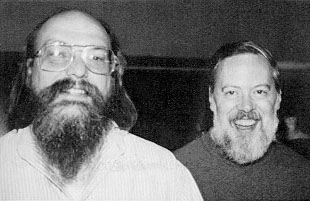
\includegraphics[width=1.\textwidth]{c-unix-authors}
		\end{column}
		
		\begin{column}{.7\textwidth}
			
			\Large
			History of C
			\normalsize
			\begin{itemize}
				\item  1969: B created, based on BCPL, to replace PDP-7 assembler as the system programming language for Unix, remained a typeless language like BCPL 
			
				
				\item 1971: NB ("new B") created when porting B to PDP-11, types (int, char, arrays and pointers), array-to-pointer conversion, compilation to machine code 
				\item 1972: Language renamed to C, structs, preprocessor, portable I/O
				\item 1973: Unix re-written in C 
				\item 1978: The C Programming Language, 1st edition 
			\end{itemize}
			
			\tiny The Development of the C Language, Dennis M. Ritchie,1993
		\end{column}
		
		
	\end{columns}
	
	
\end{frame}


%-------------------------------------------------
\begin{frame}[plain]
	\frametitle{Introduction}
	
	
	
	\begin{columns}
		
		\begin{column}{.3\textwidth}
			
			
\includegraphics[width=1.\textwidth]{clang}
			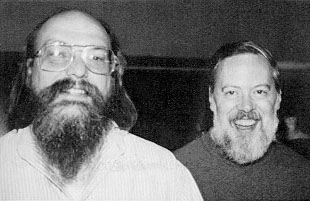
\includegraphics[width=1.\textwidth]{c-unix-authors}
		\end{column}
		
		\begin{column}{.7\textwidth}
			
			\Large
			Why was C be used to develop UNIX? \\
			C was a traditional procedural family language
			\normalsize
			\begin{itemize}
				\item  SPEED CLOSE TO ASSEMBLY
				\item  'CLOSE TO MACHINE' ABSTRACTION
				\item  TYPE SAFETY
				\item  PORTABILITY
				\item  SIMPLE/SMALL LANG \& BIG LIBRARY
				\item  the relationship between arrays and pointers
			\end{itemize}
			
		\end{column}
		
		
	\end{columns}
	
	
\end{frame}

%-------------------------------------------------
\begin{frame}[plain]
	\frametitle{Introduction}
	
	
	
	\begin{columns}
		
		\begin{column}{.3\textwidth}
			
			
\includegraphics[width=1.\textwidth]{clang}
			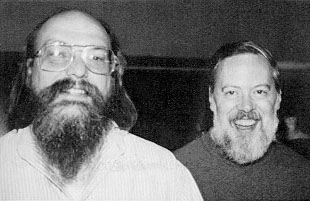
\includegraphics[width=1.\textwidth]{c-unix-authors}
		\end{column}
		
		\begin{column}{.7\textwidth}
			
			\Large
			Why was C be used to develop UNIX?
			\normalsize
			\begin{itemize}
				\item  Thompson decided that Unix possibly needed a system programming language, he created a language B(from BCPL). B can be thought of as C without types;
				\item  BCPL, B, and C all fit firmly in the traditional procedural family typified by Fortran and Algol 60. They are \textbf{'close to the machine' abstractions}.
				
				\item BCPL, B have a single data type, the `word,' or `cell,' a fixed-length bit pattern. Memory in these languages consists of a linear array of such cells.  B generated 'threaded code'.
				
				\item The C extended the B  by adding types and also rewrote its compiler to generate PDP-11 machine instructions.
				
				\item The C compiler is capable of producing programs fast and small enough to compete with assembly language.
				
				\item This DEC VAX 11/780 machine became much more popular.
			\end{itemize}
			
		\end{column}
		
		
	\end{columns}
	
	
\end{frame}

%-------------------------------------------------
\begin{frame}[plain]
	\frametitle{Introduction}
	
	
	
	\begin{columns}
		
		\begin{column}{.3\textwidth}
			
			
\includegraphics[width=1.\textwidth]{clang}
			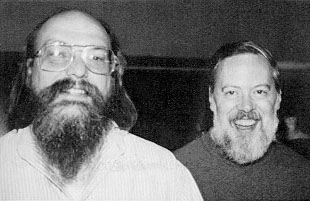
\includegraphics[width=1.\textwidth]{c-unix-authors}
		\end{column}
		
		\begin{column}{.7\textwidth}
			
			\Large
			Why was C be used to develop UNIX? \\
			C was a traditional procedural family language
			\normalsize
			\begin{itemize}
				\item  SPEED CLOSE TO ASSEMBLY
				\item  'CLOSE TO MACHINE' ABSTRACTION
				\item  TYPE SAFETY
				\item  PORTABILITY
				\item  SIMPLE/SMALL LANG \& BIG LIBRARY

			\end{itemize}
			
		\end{column}
		
		
	\end{columns}
	
	
\end{frame}

%-------------------------------------------------
\begin{frame}[plain]
	\frametitle{Introduction}
	
	
	
	\begin{columns}
		
		\begin{column}{.3\textwidth}
			
			
\includegraphics[width=1.\textwidth]{clang}
			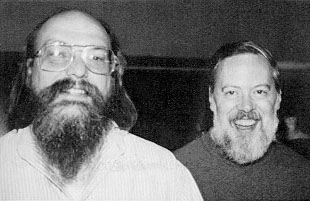
\includegraphics[width=1.\textwidth]{c-unix-authors}
		\end{column}
		
		\begin{column}{.7\textwidth}
			
			\Large
			Whence Success? 
			
			\normalsize
			\begin{itemize}
				\item  The success of Unix itself was the most important factor
				\item  Remains a simple and small language
				\item  At the same time the language is sufficiently abstracted from machine details that program portability can be achieved
				\item  C and its central library support always remained in touch with a real environment
				\item The actual C language as seen by millions of users using many different compilers has remained remarkably stable and unified compared to those of similarly widespread currency,for example Pascal and Fortran.
			\end{itemize}
			
		\end{column}
		
		
	\end{columns}
	
	
\end{frame}


%-------------------------------------------------
\begin{frame}[plain]
	\frametitle{A Study of the Unix Operating System 1973–2015}
	
	
	
	\begin{columns}
		
		\begin{column}{.3\textwidth}
			
			
\includegraphics[width=1.\textwidth]{clang}
			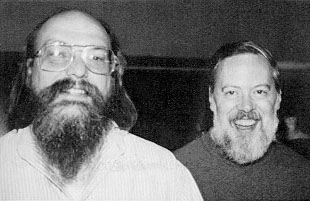
\includegraphics[width=1.\textwidth]{c-unix-authors}
		\end{column}
		
		\begin{column}{.7\textwidth}
			
			\LARGE
			\begin{block}{objective}
			The objective of this work is to study the long term evo-
			lution of C programming in the context of the Unix oper-
			ating system development. 
			\end{block}
		
			Formulate seven hypotheses associated with the long term evolution of C programming in		the Unix operating system

			
		\end{column}
		
		
	\end{columns}
	
	
\end{frame}


%-------------------------------------------------
\begin{frame}[plain]
	\frametitle{A Study of the Unix Operating System 1973–2015}
	
	
	
	\begin{columns}
		
		\begin{column}{.3\textwidth}
			
			
\includegraphics[width=1.\textwidth]{clang}
			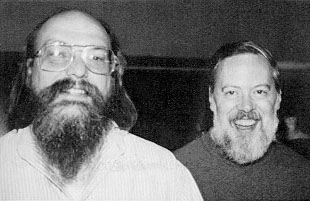
\includegraphics[width=1.\textwidth]{c-unix-authors}
		\end{column}
		
		\begin{column}{.7\textwidth}
			
			
			Seven hypotheses associated with the long term evolution of C programming in		the Unix operating system
			
			\begin{itemize}
				\item  Programming practices reflect technology affordances
				
				\item  Modularity increases with code size
				
				\item  New language features are increasingly used
				to saturation point
				
				
				\item  Programmers trust the compiler for register
				allocation
				
				\item Code formatting practices converge to a com-
				mon standard
				
				\item  Software complexity evolution follows self cor-
				rection feedback mechanisms
				
				\item Code readability increases
				
			\end{itemize}
			
		\end{column}
		
		
	\end{columns}
	
	
\end{frame}


%-------------------------------------------------
\begin{frame}[plain]
	\frametitle{A Study of the Unix Operating System 1973–2015}
	Timeline of indicative analyzed revisions and milestones in (from top to bottom): C language evolution, developer interfaces, programming guidelines, processing capacity, collaboration mechanisms, and tools.
	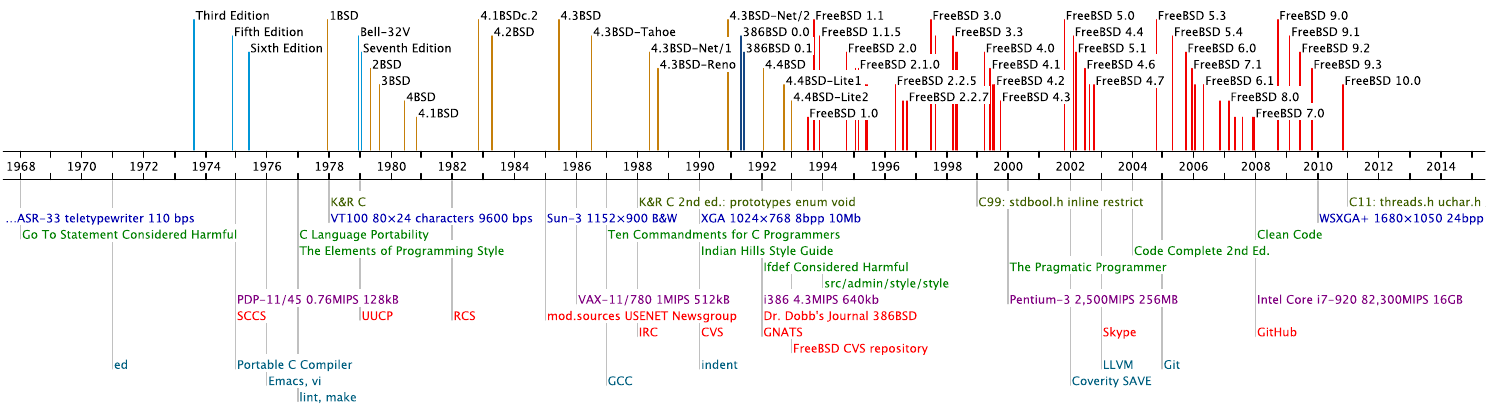
\includegraphics[width=1.6\textwidth]{c-unix-analysis}
	
\end{frame}	


%-------------------------------------------------
\begin{frame}[plain]
	\frametitle{A Study of the Unix Operating System 1973–2015}
	\centering
H1: Programming practices reflect
technology affordances

	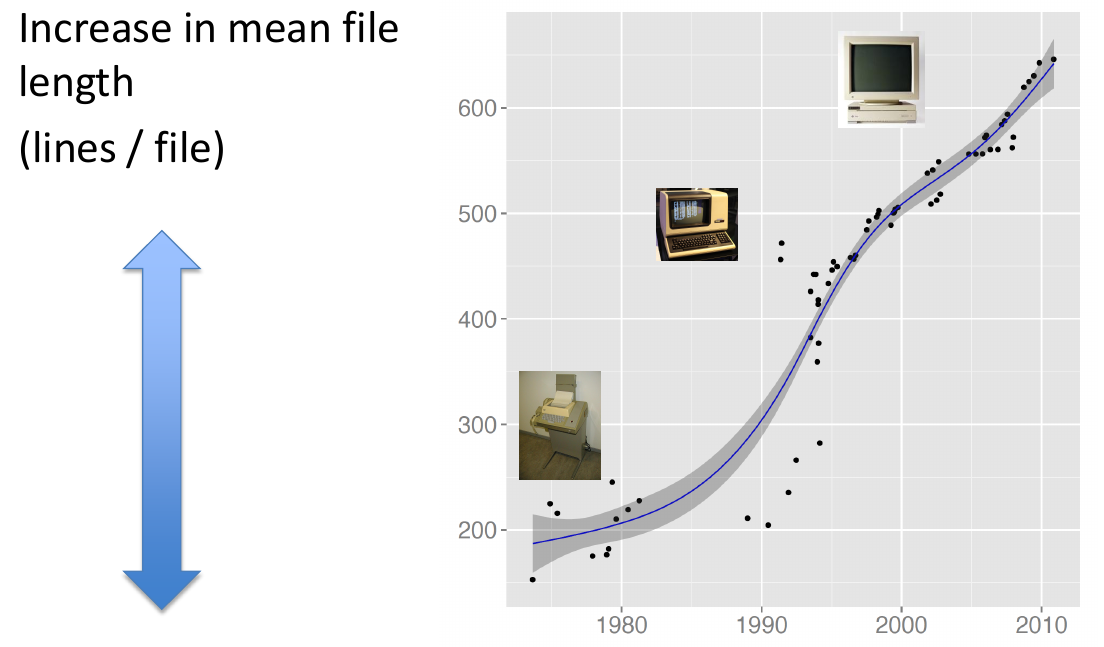
\includegraphics[width=.8\textwidth]{h1-ana-1}
	
	\tiny Half Century of Unix:
	History, Preservation, and
	Lessons Learned,Diomidis Spinellis, keynote of OW2 Consortium, 2017
\end{frame}	


%-------------------------------------------------
\begin{frame}[plain]
	\frametitle{A Study of the Unix Operating System 1973–2015}
	\centering
	H1: Programming practices reflect
	technology affordances
	
	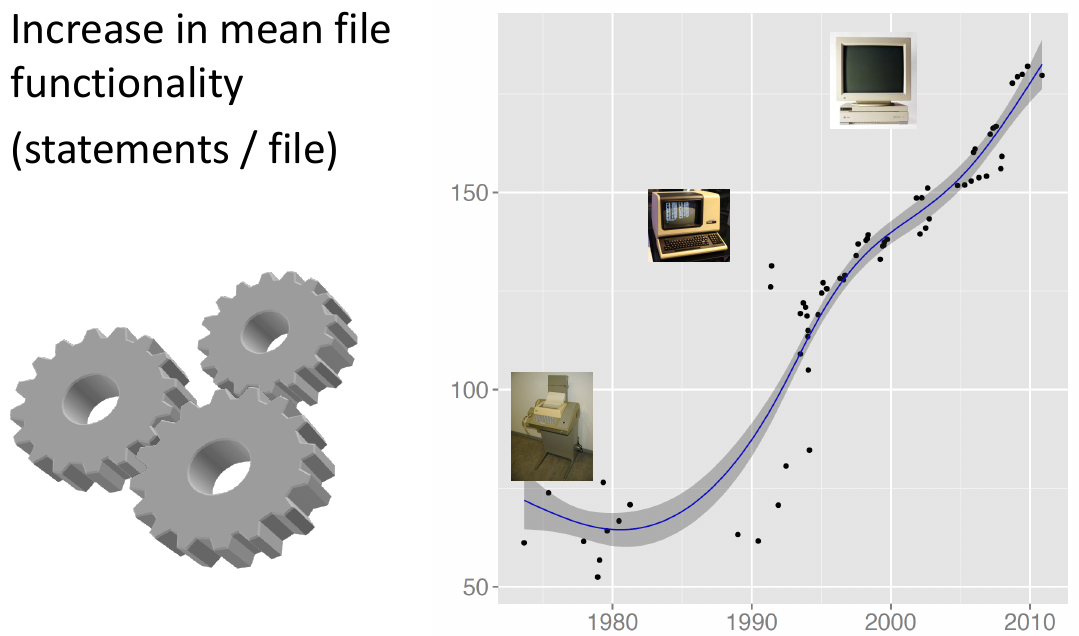
\includegraphics[width=.8\textwidth]{h1-ana-2}

	\tiny Half Century of Unix:
History, Preservation, and
Lessons Learned,Diomidis Spinellis, keynote of OW2 Consortium, 2017
	
\end{frame}	


%-------------------------------------------------
\begin{frame}[plain]
	\frametitle{A Study of the Unix Operating System 1973–2015}
	\centering
	H1: Programming practices reflect
	technology affordances
	
	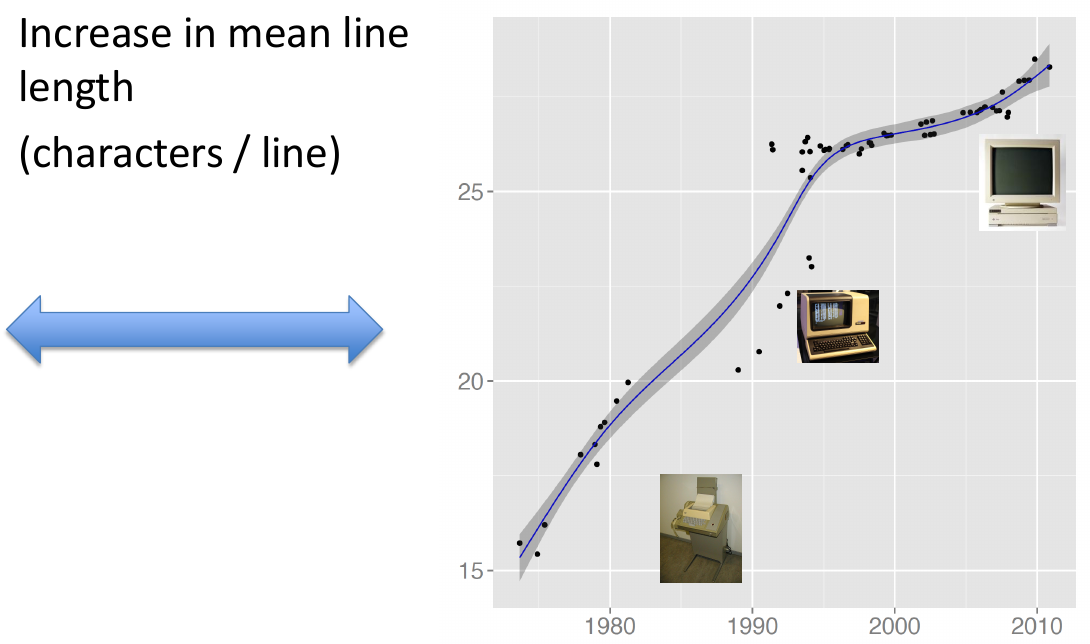
\includegraphics[width=.8\textwidth]{h1-ana-3}

	\tiny Half Century of Unix:
History, Preservation, and
Lessons Learned,Diomidis Spinellis, keynote of OW2 Consortium, 2017
	
\end{frame}	


%-------------------------------------------------
\begin{frame}[plain]
	\frametitle{A Study of the Unix Operating System 1973–2015}
	\centering
	H1: Programming practices reflect
	technology affordances
	
	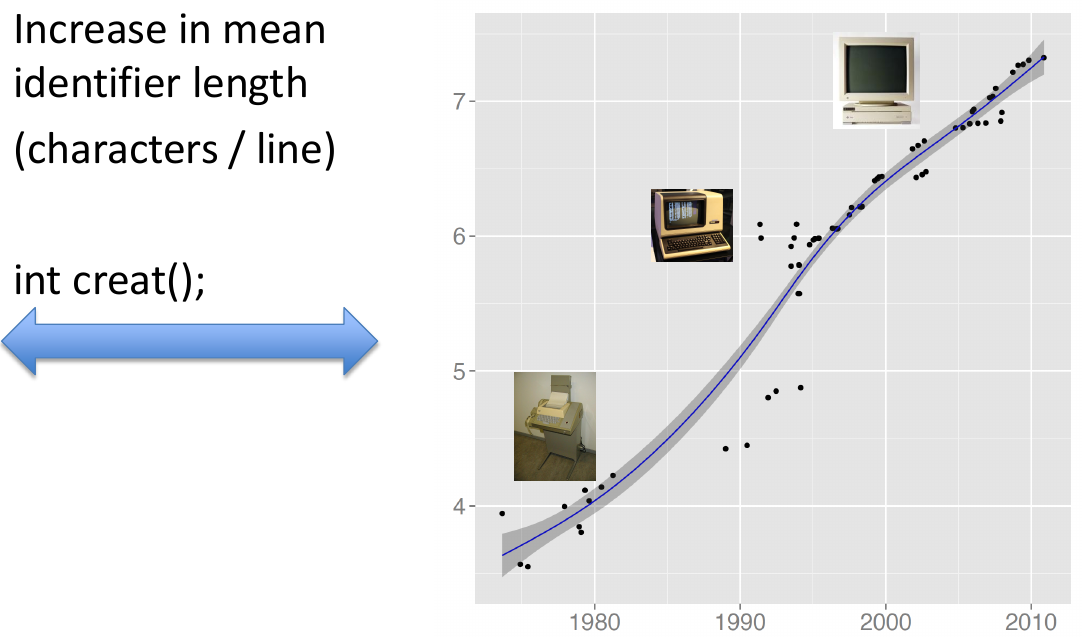
\includegraphics[width=.8\textwidth]{h1-ana-4}

	\tiny Half Century of Unix:
History, Preservation, and
Lessons Learned,Diomidis Spinellis, keynote of OW2 Consortium, 2017
	
\end{frame}	



%-------------------------------------------------
\begin{frame}[plain]
	\frametitle{A Study of the Unix Operating System 1973–2015}
	\centering
	H1: Programming practices reflect
	technology affordances
	
	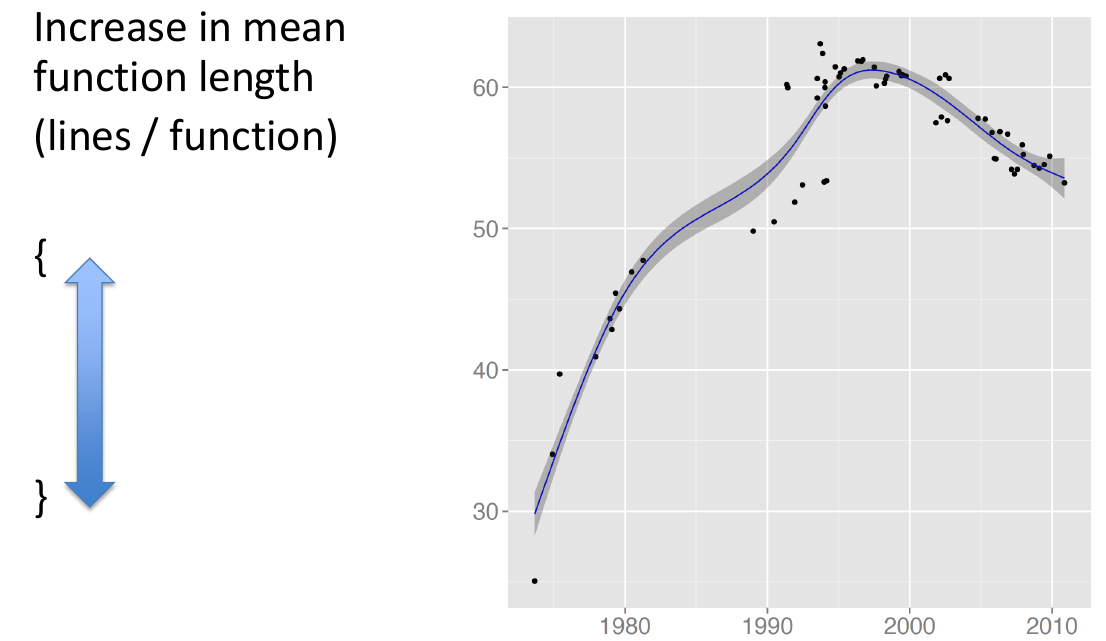
\includegraphics[width=.8\textwidth]{h1-ana-5}
	
	\tiny Half Century of Unix:
	History, Preservation, and
	Lessons Learned,Diomidis Spinellis, keynote of OW2 Consortium, 2017
	
\end{frame}	



%-------------------------------------------------
\begin{frame}[plain]
	\frametitle{A Study of the Unix Operating System 1973–2015}
	\centering
	H2: Modularity increases with code
	size
	
	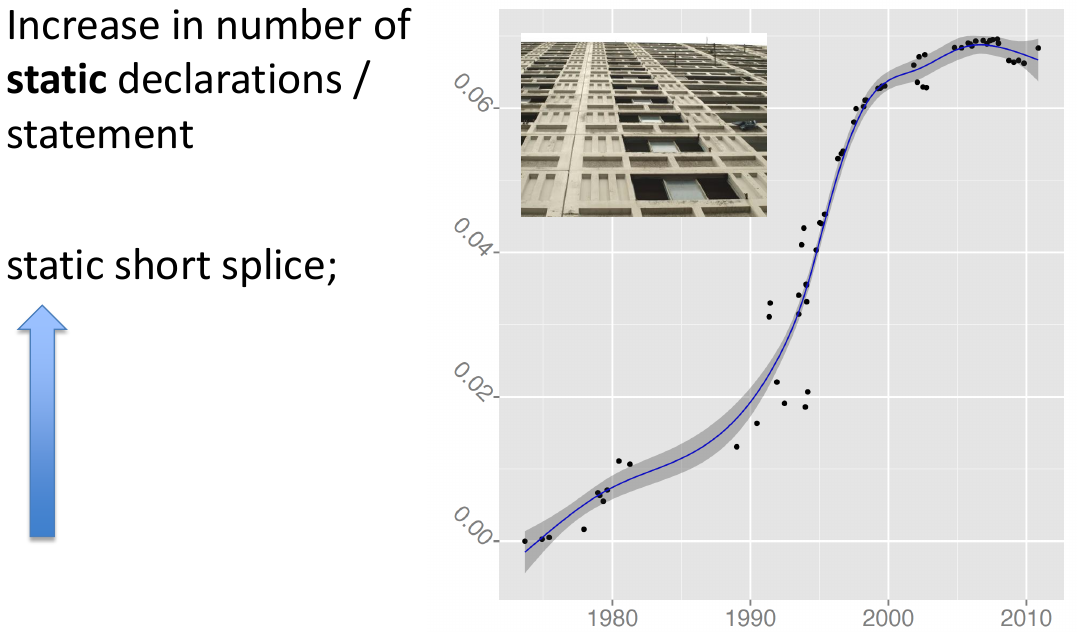
\includegraphics[width=.8\textwidth]{h2-ana-1}
	
	\tiny Half Century of Unix:
	History, Preservation, and
	Lessons Learned,Diomidis Spinellis, keynote of OW2 Consortium, 2017
	
\end{frame}	



%-------------------------------------------------
\begin{frame}[plain]
	\frametitle{A Study of the Unix Operating System 1973–2015}
	\centering
	H2: Modularity increases with code
	size
	
	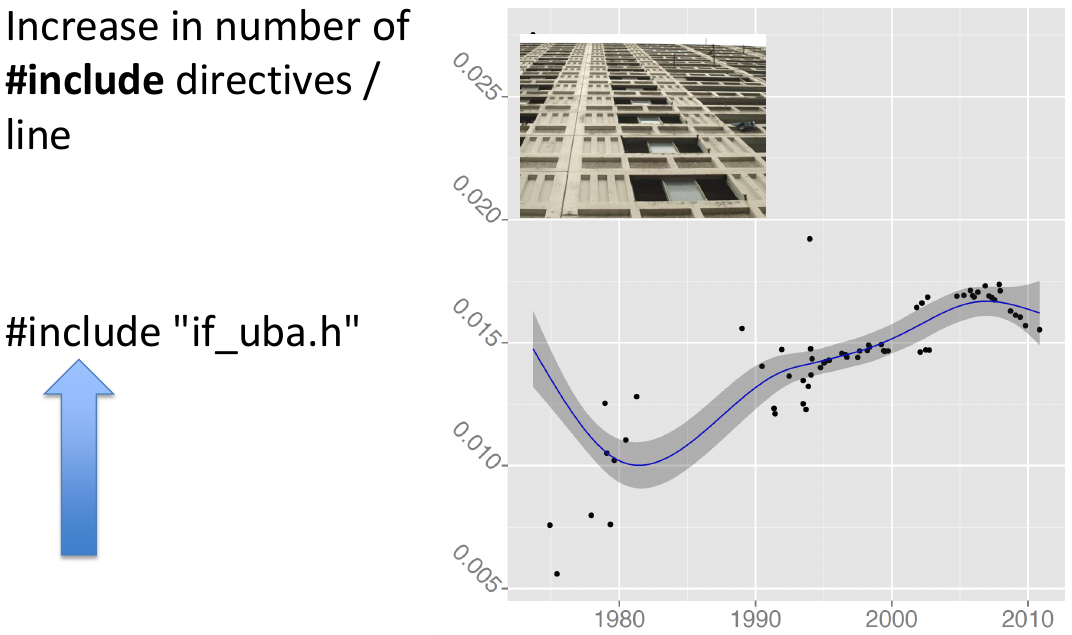
\includegraphics[width=.8\textwidth]{h2-ana-2}
	
	\tiny Half Century of Unix:
	History, Preservation, and
	Lessons Learned,Diomidis Spinellis, keynote of OW2 Consortium, 2017
	
\end{frame}	




%-------------------------------------------------
\begin{frame}[plain]
	\frametitle{A Study of the Unix Operating System 1973–2015}
	\centering
	H3: New language features are
	increasingly used to saturation point
	
	
	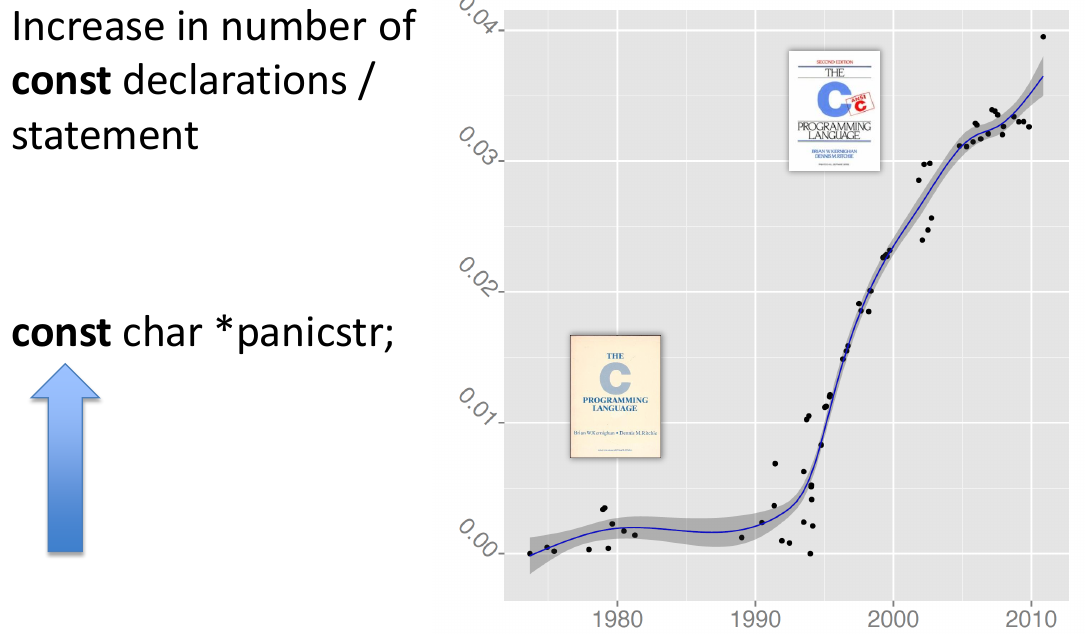
\includegraphics[width=.8\textwidth]{h3-ana-1}
	
	\tiny Half Century of Unix:
	History, Preservation, and
	Lessons Learned,Diomidis Spinellis, keynote of OW2 Consortium, 2017
	
\end{frame}	

%-------------------------------------------------
\begin{frame}[plain]
	\frametitle{A Study of the Unix Operating System 1973–2015}
	\centering
	H3: New language features are
	increasingly used to saturation point
	
	
	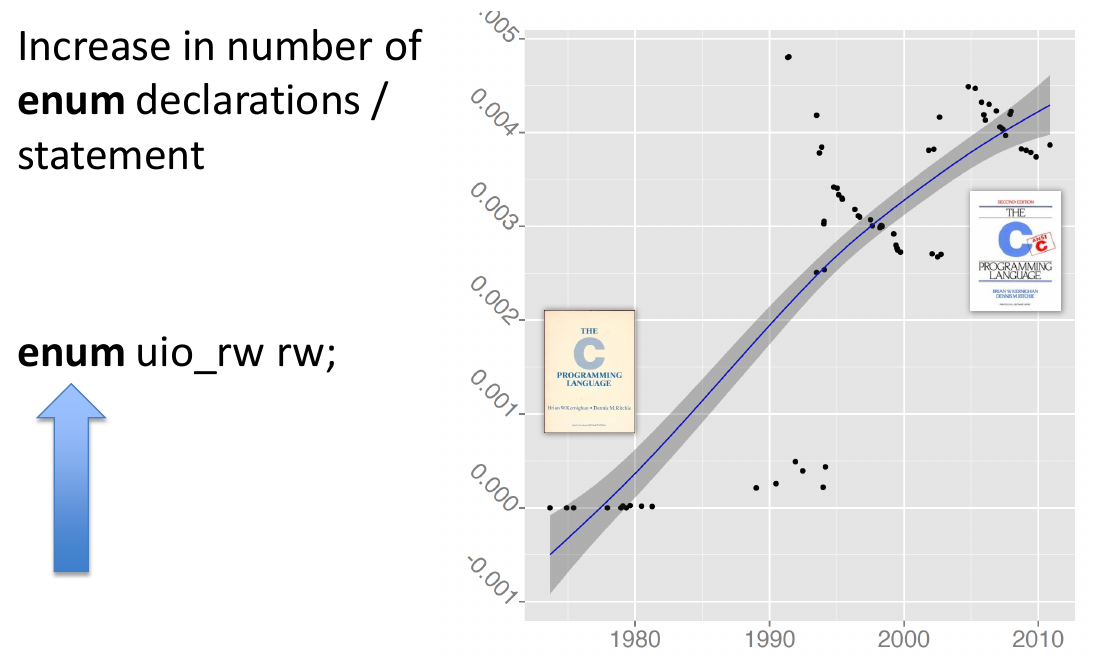
\includegraphics[width=.8\textwidth]{h3-ana-2}
	
	\tiny Half Century of Unix:
	History, Preservation, and
	Lessons Learned,Diomidis Spinellis, keynote of OW2 Consortium, 2017
	
\end{frame}	

%-------------------------------------------------
\begin{frame}[plain]
	\frametitle{A Study of the Unix Operating System 1973–2015}
	\centering
	H3: New language features are
	increasingly used to saturation point
	
	
	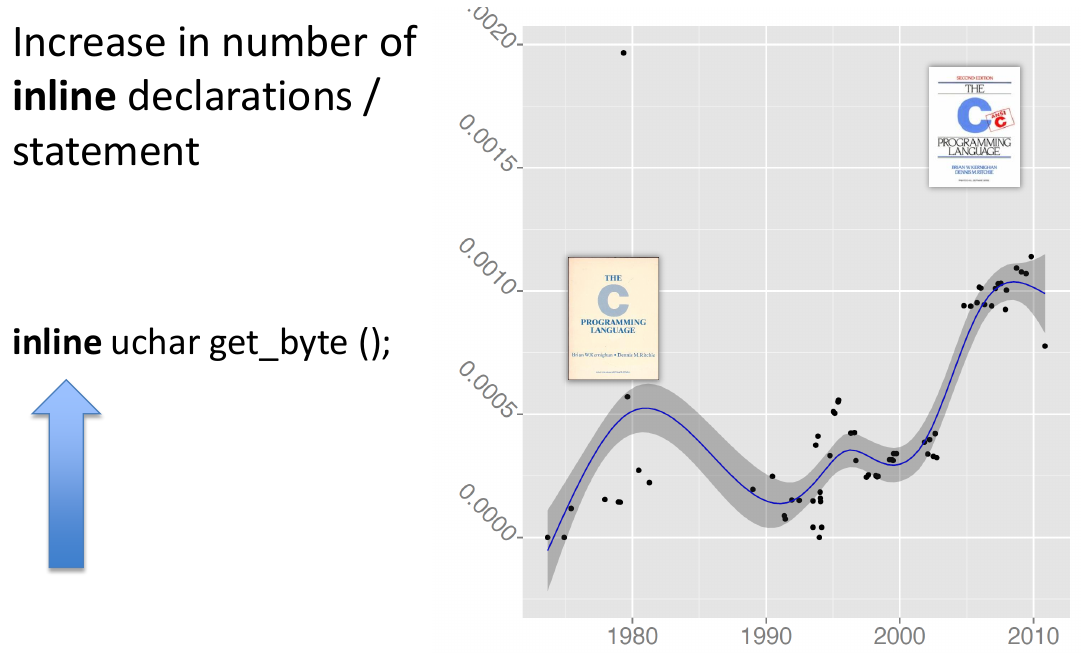
\includegraphics[width=.8\textwidth]{h3-ana-3}
	
	\tiny Half Century of Unix:
	History, Preservation, and
	Lessons Learned,Diomidis Spinellis, keynote of OW2 Consortium, 2017
	
\end{frame}	

%-------------------------------------------------
\begin{frame}[plain]
	\frametitle{A Study of the Unix Operating System 1973–2015}
	\centering
	H3: New language features are
	increasingly used to saturation point
	
	
	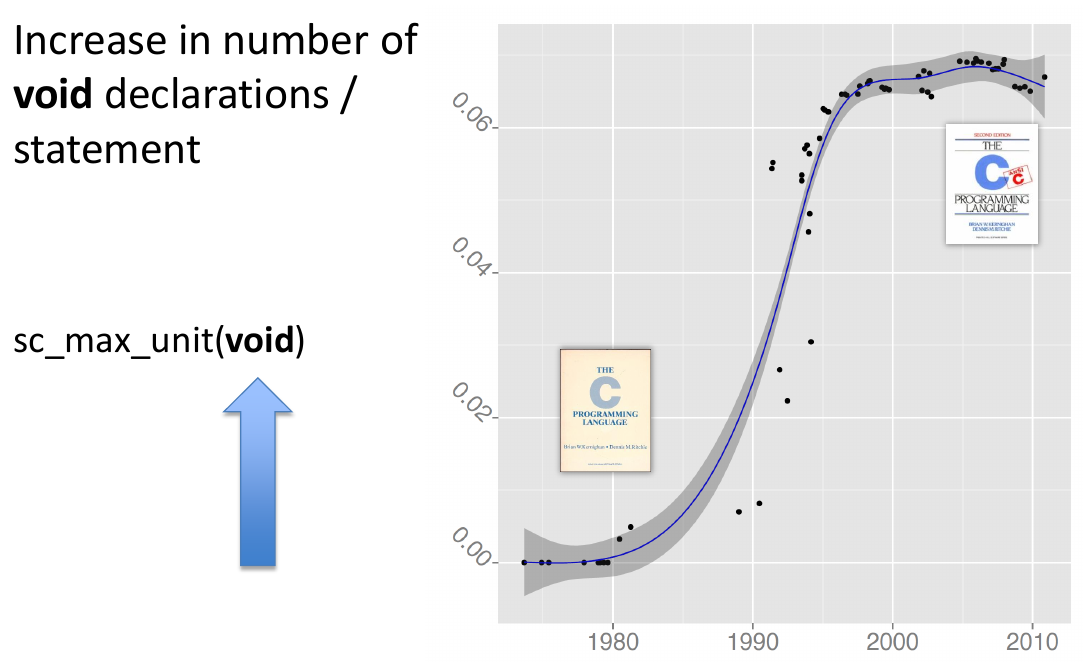
\includegraphics[width=.8\textwidth]{h3-ana-4}
	
	\tiny Half Century of Unix:
	History, Preservation, and
	Lessons Learned,Diomidis Spinellis, keynote of OW2 Consortium, 2017
	
\end{frame}	

%-------------------------------------------------
\begin{frame}[plain]
	\frametitle{A Study of the Unix Operating System 1973–2015}
	\centering
	H3: New language features are
	increasingly used to saturation point
	
	
	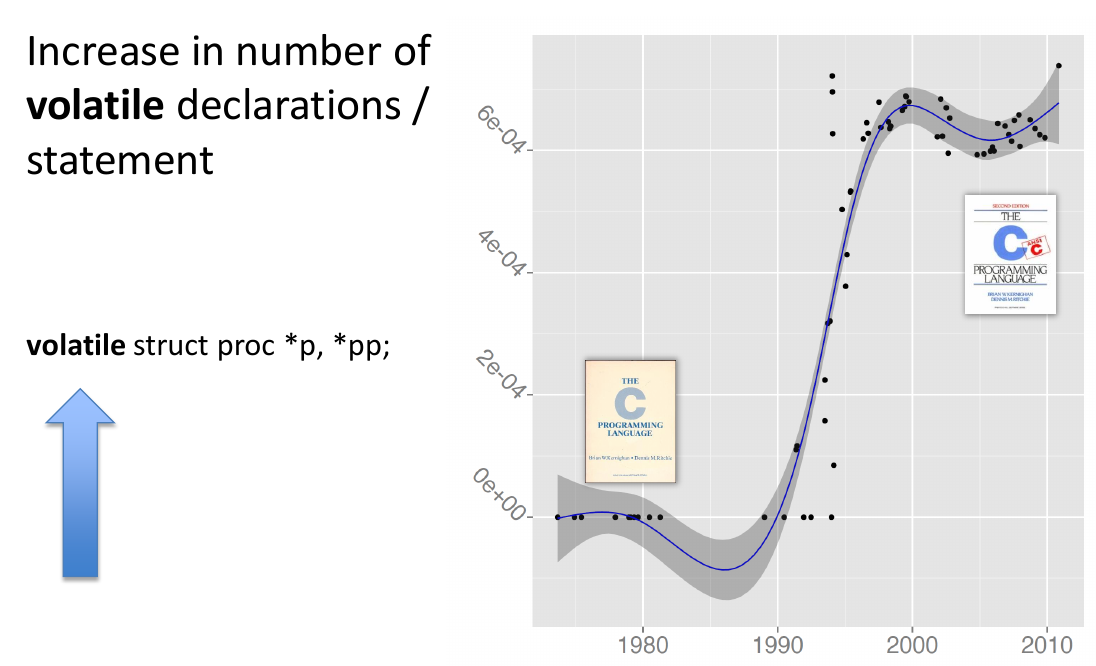
\includegraphics[width=.8\textwidth]{h3-ana-5}
	
	\tiny Half Century of Unix:
	History, Preservation, and
	Lessons Learned,Diomidis Spinellis, keynote of OW2 Consortium, 2017
	
\end{frame}	

%-------------------------------------------------
\begin{frame}[plain]
	\frametitle{A Study of the Unix Operating System 1973–2015}
	\centering
	H3: New language features are
	increasingly used to saturation point
	
	
	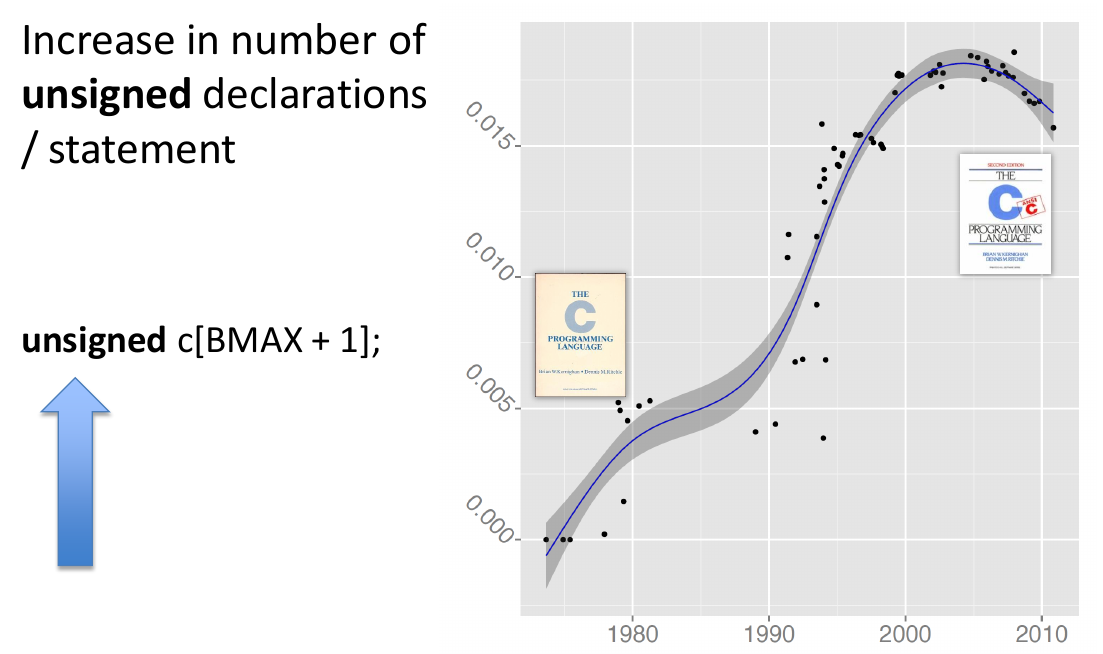
\includegraphics[width=.8\textwidth]{h3-ana-6}
	
	\tiny Half Century of Unix:
	History, Preservation, and
	Lessons Learned,Diomidis Spinellis, keynote of OW2 Consortium, 2017
	
\end{frame}	


%-------------------------------------------------
\begin{frame}[plain]
	\frametitle{A Study of the Unix Operating System 1973–2015}
	\centering
	H4: Programmers trust the compiler
	for register allocation
	
	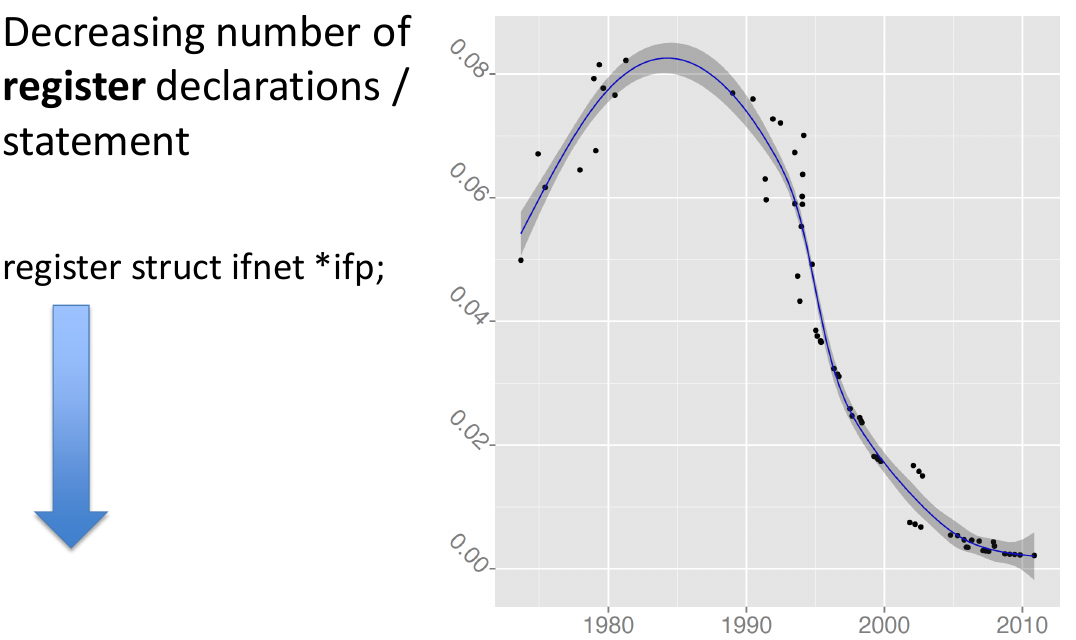
\includegraphics[width=.8\textwidth]{h4-ana-1}
	
	\tiny Half Century of Unix:
	History, Preservation, and
	Lessons Learned,Diomidis Spinellis, keynote of OW2 Consortium, 2017
	
\end{frame}	

%-------------------------------------------------
\begin{frame}[plain]
	\frametitle{A Study of the Unix Operating System 1973–2015}
	\centering
	H5: Code formatting practices
	converge to a common standard
	
	
	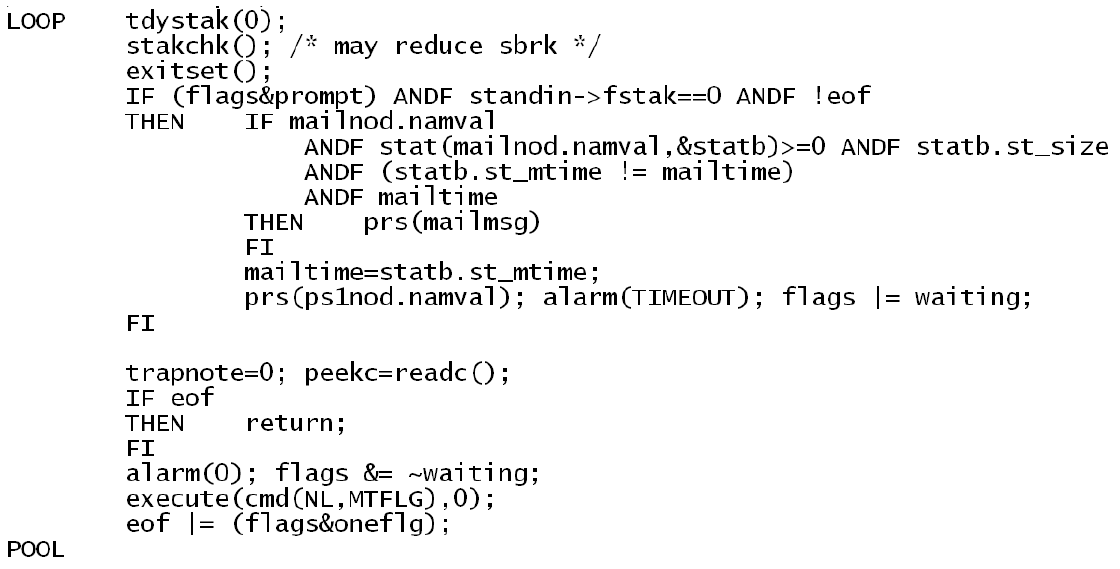
\includegraphics[width=.8\textwidth]{h5-ana-1}
	
	\tiny Half Century of Unix:
	History, Preservation, and
	Lessons Learned,Diomidis Spinellis, keynote of OW2 Consortium, 2017
	
\end{frame}	

%-------------------------------------------------
\begin{frame}[plain]
	\frametitle{A Study of the Unix Operating System 1973–2015}
	\centering
	H5: Code formatting practices
	converge to a common standard
	
	
	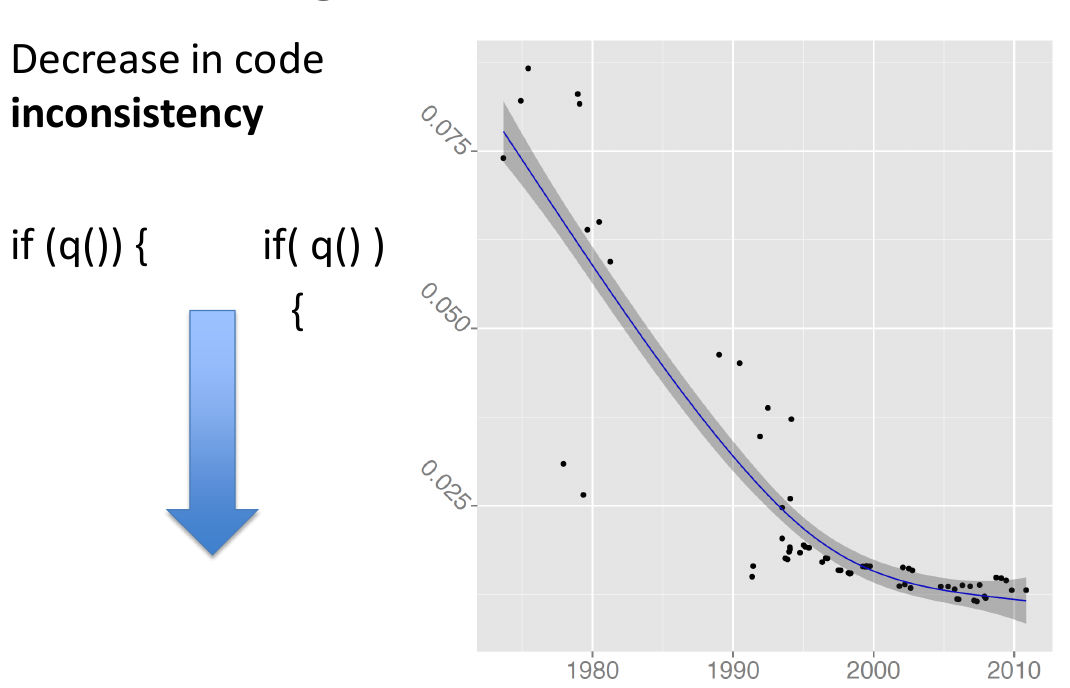
\includegraphics[width=.8\textwidth]{h5-ana-2}
	
	\tiny Half Century of Unix:
	History, Preservation, and
	Lessons Learned,Diomidis Spinellis, keynote of OW2 Consortium, 2017
	
\end{frame}	


%-------------------------------------------------
\begin{frame}[plain]
	\frametitle{A Study of the Unix Operating System 1973–2015}
	\centering
	H5: Code formatting practices
	converge to a common standard
	
	
	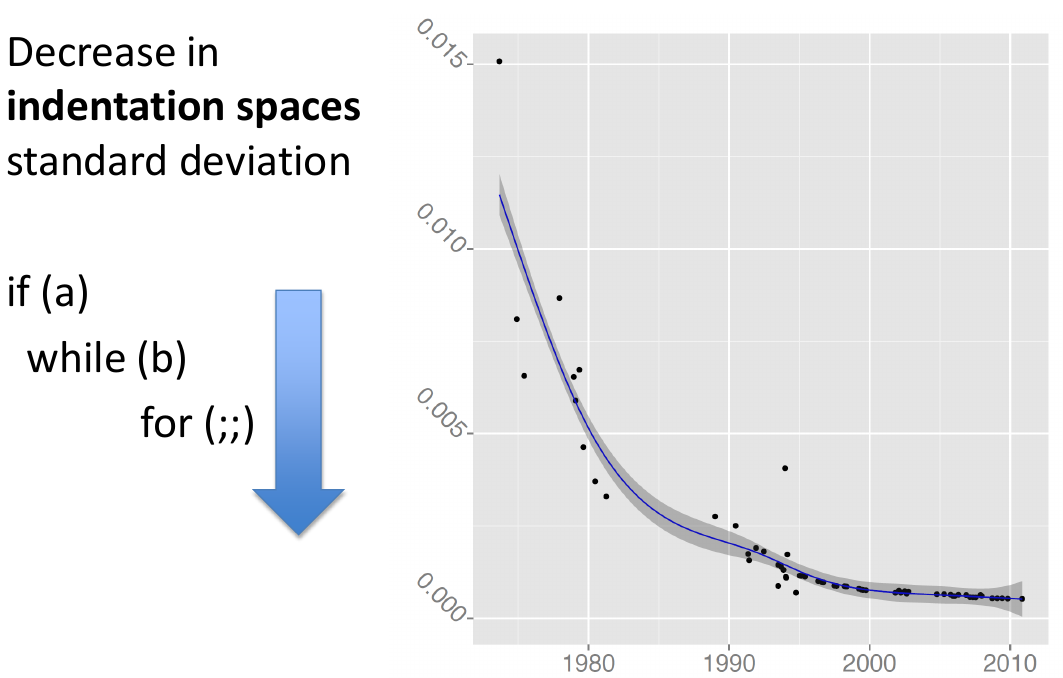
\includegraphics[width=.8\textwidth]{h5-ana-3}
	
	\tiny Half Century of Unix:
	History, Preservation, and
	Lessons Learned,Diomidis Spinellis, keynote of OW2 Consortium, 2017
	
\end{frame}	




%-------------------------------------------------
\begin{frame}[plain]
	\frametitle{A Study of the Unix Operating System 1973–2015}
	\centering
	H6: Software complexity evolution
	follows self correction

	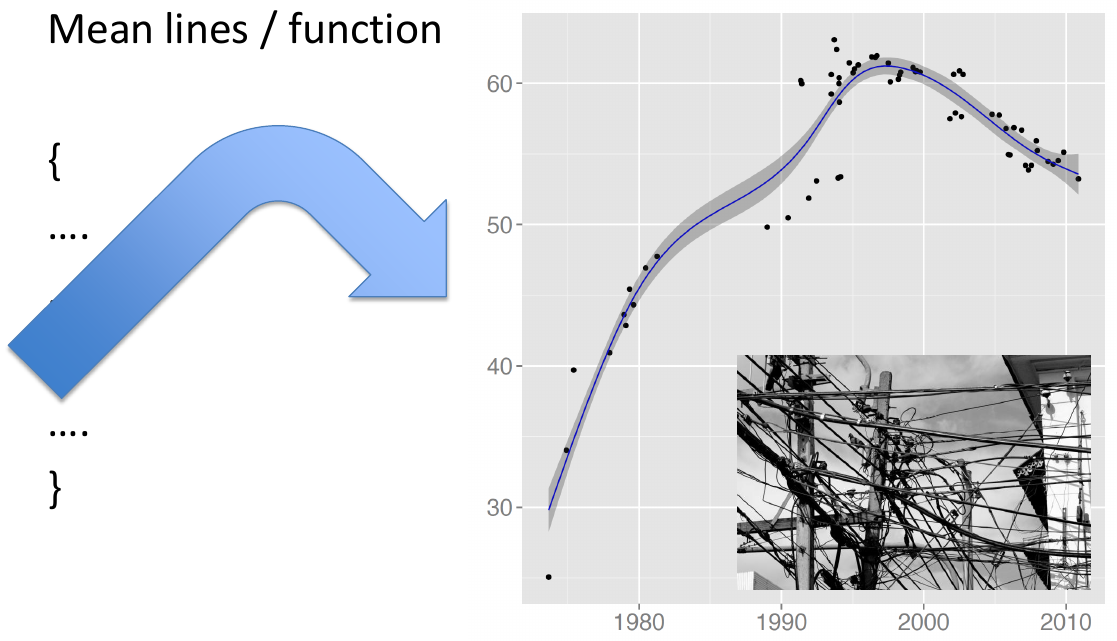
\includegraphics[width=.8\textwidth]{h6-ana-1}
	
	\tiny Half Century of Unix:
	History, Preservation, and
	Lessons Learned,Diomidis Spinellis, keynote of OW2 Consortium, 2017
	
\end{frame}	

%-------------------------------------------------
\begin{frame}[plain]
	\frametitle{A Study of the Unix Operating System 1973–2015}
	\centering
	H6: Software complexity evolution
	follows self correction
	
	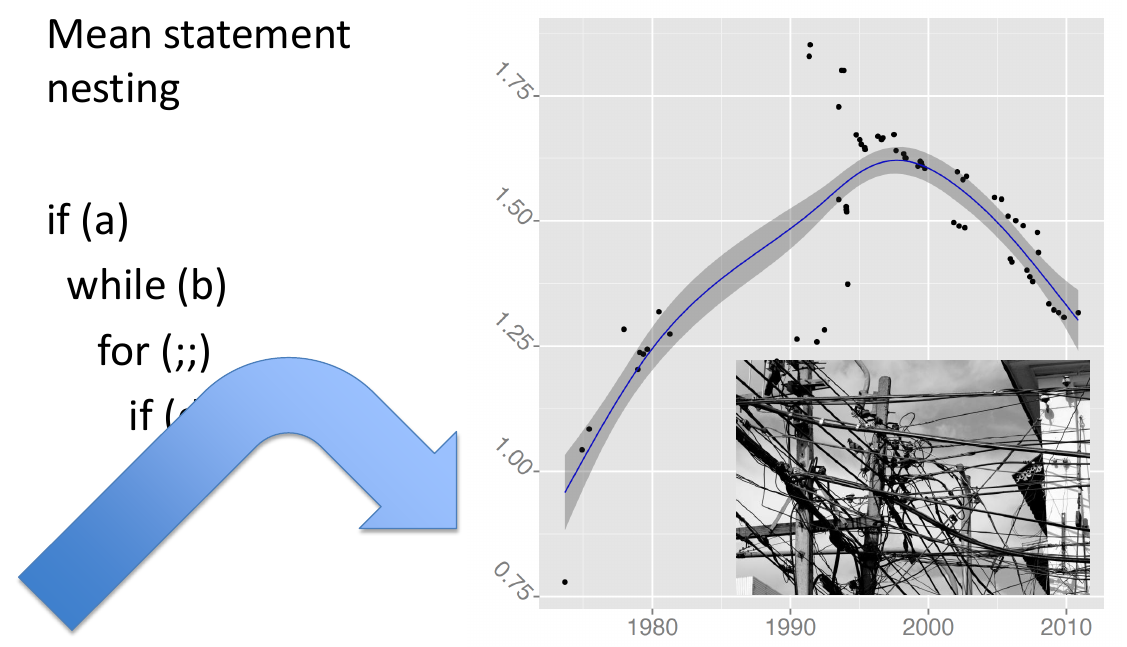
\includegraphics[width=.8\textwidth]{h6-ana-2}
	
	\tiny Half Century of Unix:
	History, Preservation, and
	Lessons Learned,Diomidis Spinellis, keynote of OW2 Consortium, 2017
	
\end{frame}	


%-------------------------------------------------
\begin{frame}[plain]
	\frametitle{A Study of the Unix Operating System 1973–2015}
	\centering
	H6: Software complexity evolution
	follows self correction
	
	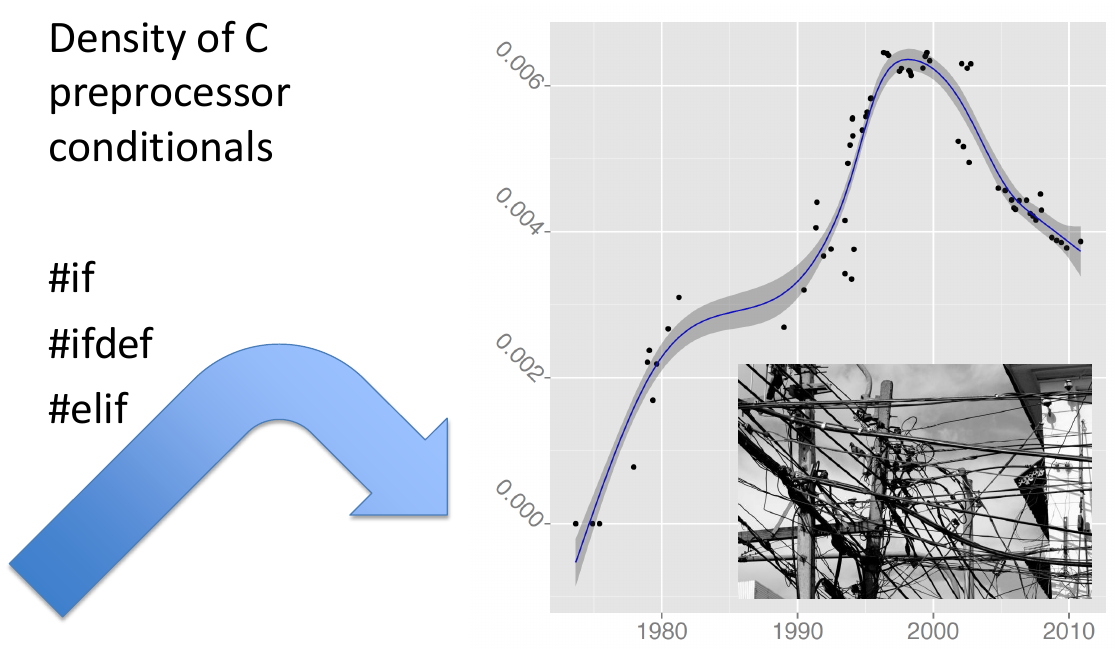
\includegraphics[width=.8\textwidth]{h6-ana-3}
	
	\tiny Half Century of Unix:
	History, Preservation, and
	Lessons Learned,Diomidis Spinellis, keynote of OW2 Consortium, 2017
	
\end{frame}	



%-------------------------------------------------
\begin{frame}[plain]
	\frametitle{A Study of the Unix Operating System 1973–2015}
	\centering
	H6: Software complexity evolution
	follows self correction
	
	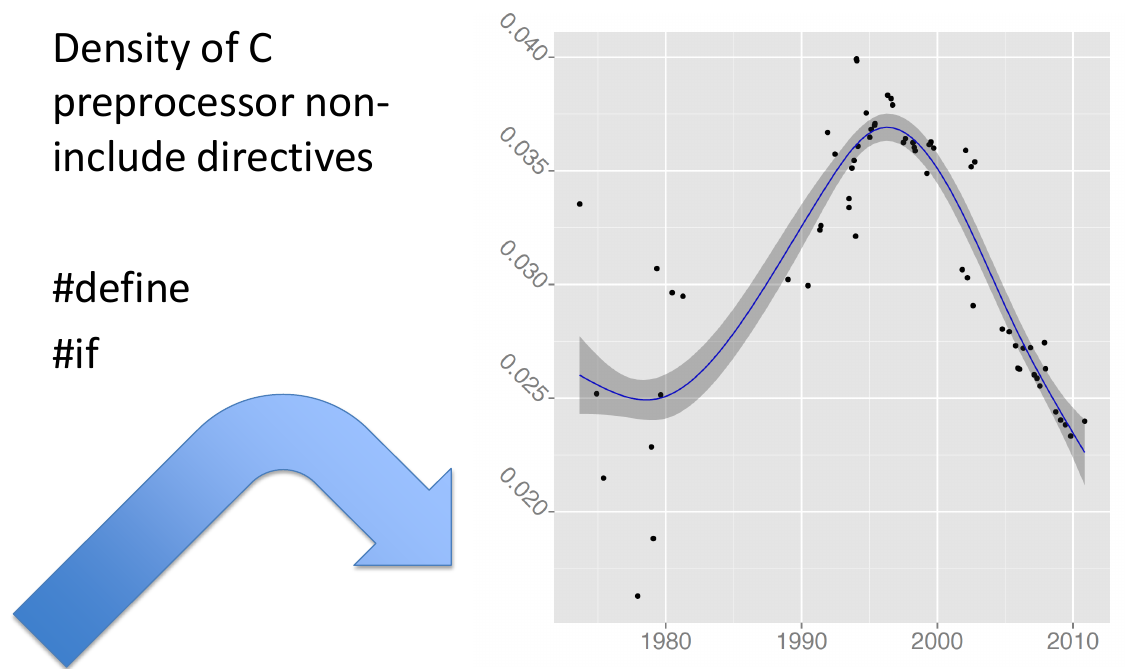
\includegraphics[width=.8\textwidth]{h6-ana-4}
	
	\tiny Half Century of Unix:
	History, Preservation, and
	Lessons Learned,Diomidis Spinellis, keynote of OW2 Consortium, 2017
	
\end{frame}	


%-------------------------------------------------
\begin{frame}[plain]
	\frametitle{A Study of the Unix Operating System 1973–2015}
	\centering
	H6: Software complexity evolution
	follows self correction
	
	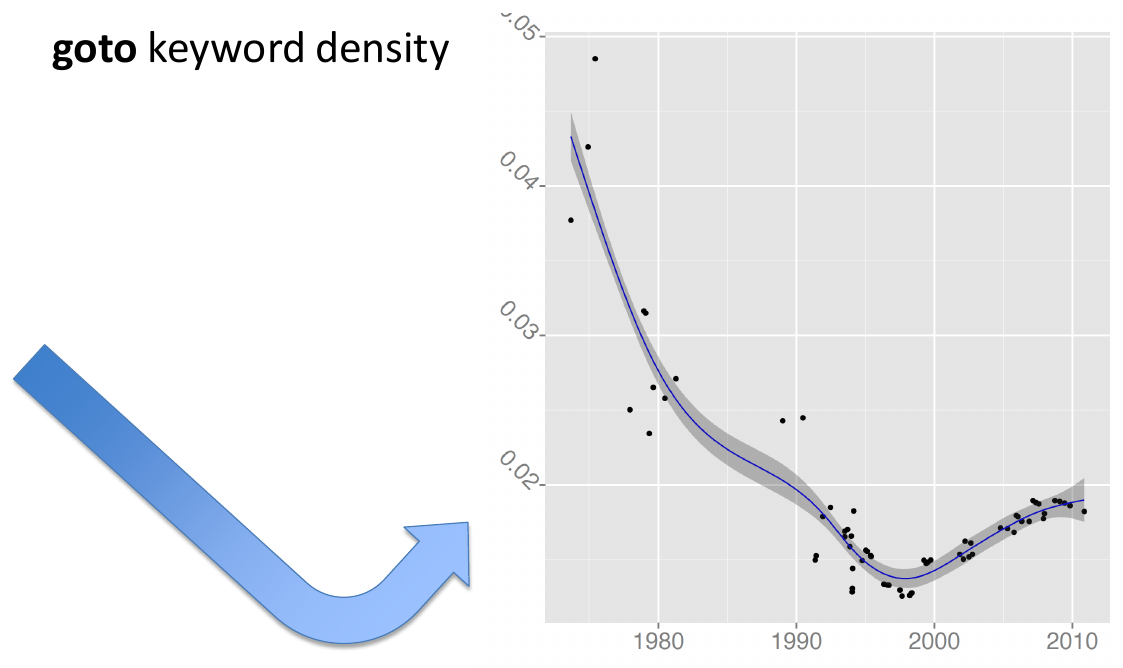
\includegraphics[width=.8\textwidth]{h6-ana-5}
	
	\tiny Half Century of Unix:
	History, Preservation, and
	Lessons Learned,Diomidis Spinellis, keynote of OW2 Consortium, 2017
	
\end{frame}	



%-------------------------------------------------
\begin{frame}[plain]
	\frametitle{A Study of the Unix Operating System 1973–2015}
	\centering
	H7: Code readability increases
	
	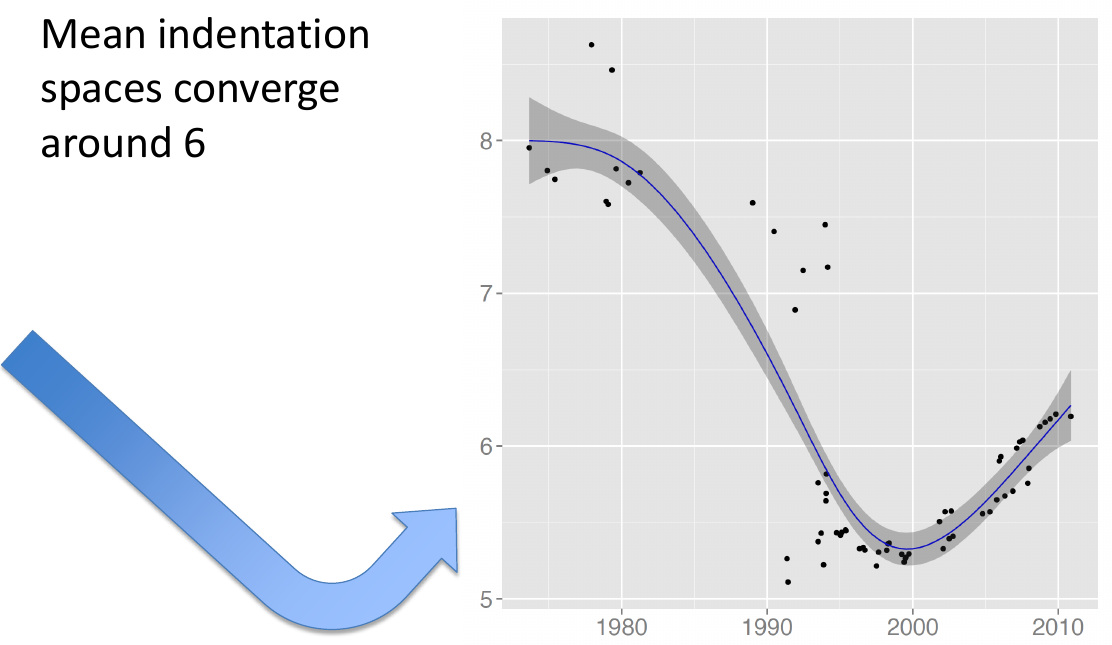
\includegraphics[width=.8\textwidth]{h7-ana-1}
	
	\tiny Half Century of Unix:
	History, Preservation, and
	Lessons Learned,Diomidis Spinellis, keynote of OW2 Consortium, 2017
	
\end{frame}

%-------------------------------------------------
\begin{frame}[plain]
	\frametitle{A Study of the Unix Operating System 1973–2015}
	\centering
	H7: Code readability increases
	
	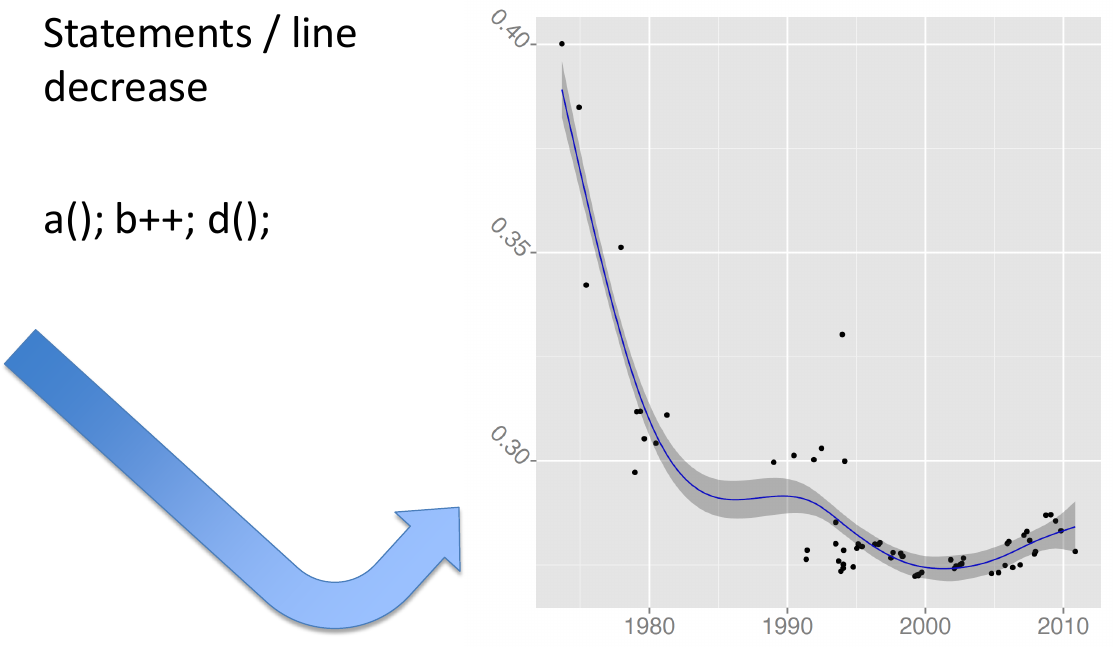
\includegraphics[width=.8\textwidth]{h7-ana-2}
	
	\tiny Half Century of Unix:
	History, Preservation, and
	Lessons Learned,Diomidis Spinellis, keynote of OW2 Consortium, 2017
	
\end{frame}

%-------------------------------------------------
\begin{frame}[plain]
	\frametitle{A Study of the Unix Operating System 1973–2015}
	\centering
	H7: Code readability increases
	
	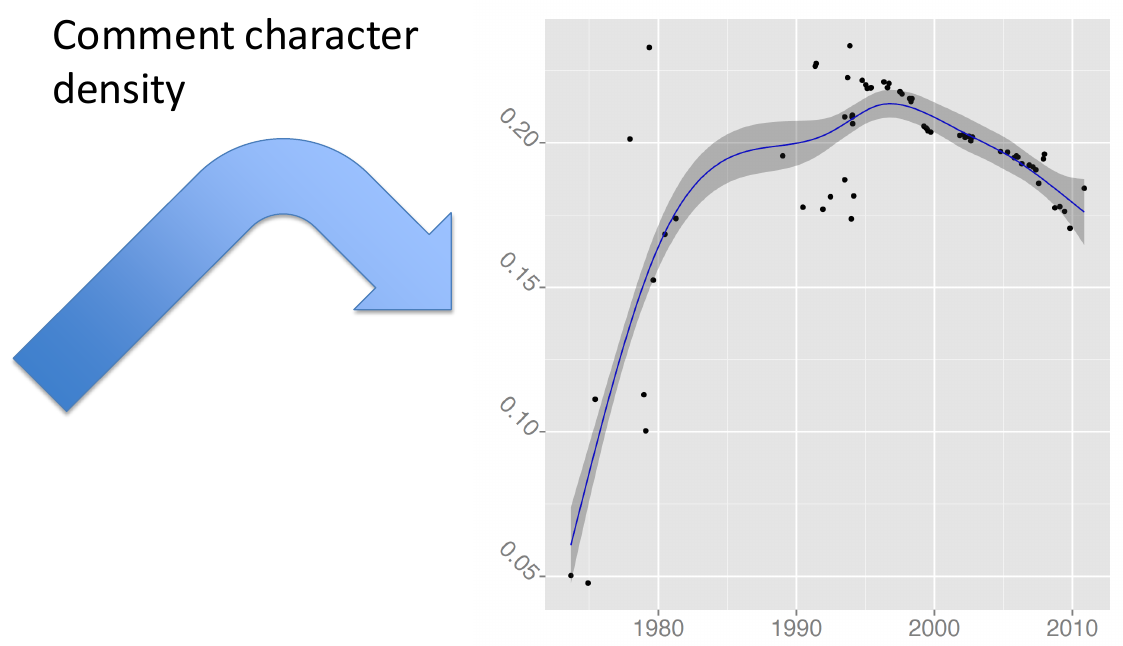
\includegraphics[width=.8\textwidth]{h7-ana-3}
	
	\tiny Half Century of Unix:
	History, Preservation, and
	Lessons Learned,Diomidis Spinellis, keynote of OW2 Consortium, 2017
	
\end{frame}


%-------------------------------------------------
\begin{frame}[plain]
	\frametitle{A Study of the Unix Operating System 1973–2015}
	\centering
	H7: Code readability increases
	
	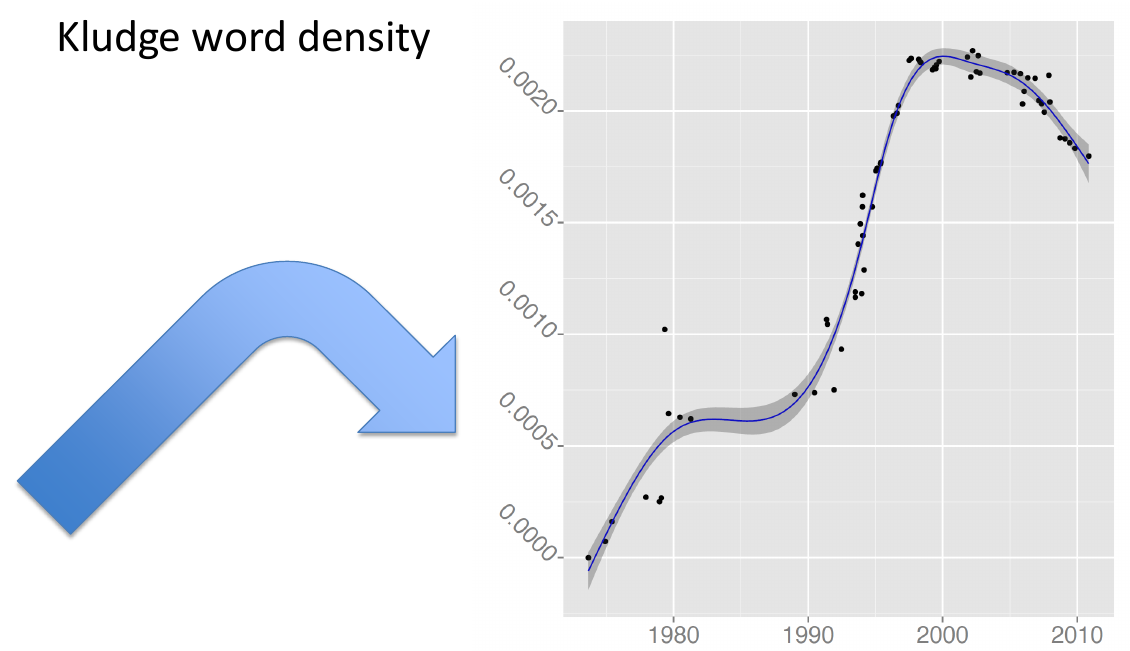
\includegraphics[width=.8\textwidth]{h7-ana-4}
	
	\tiny Half Century of Unix:
	History, Preservation, and
	Lessons Learned,Diomidis Spinellis, keynote of OW2 Consortium, 2017
	
\end{frame}
%-------------------------------------------------


%-------------------------------------------------
\begin{frame}[plain]
	\frametitle{References}
	
	\begin{itemize}
		\item The Development of the C Language, Dennis M. Ritchie,1993
		\item  An empirical study of operating systems errors, SOSP 2003
		\item Linux kernel vulnerabilities: State-of-the-art defenses and open problems,APSYS 2011
		\item  Faults in linux: ten years later,ASPLOS 2011
		\item The Evolution of C Programming Practices:
		A Study of the Unix Operating System 1973–2015, Diomidis Spinellis,
		ICSE, 2016
		
		\item Half Century of Unix:
		History, Preservation, and
		Lessons Learned,Diomidis Spinellis, keynote of OW2 Consortium, 2017
		
	\end{itemize}
	
	
\end{frame}
%-------------------------------------------------
\end{document}